\documentclass[conference]{IEEEtran}
\IEEEoverridecommandlockouts
% The preceding line is only needed to identify funding in the first footnote. If that is unneeded, please comment it out.

% IEEE CASCON 2025 Camera-Ready Copyright Notice
% Paper ID: SP-217
\IEEEpubid{\makebox[\columnwidth]{979-8-3503-8285-7/25/\$31.00~\copyright~2025~IEEE \hfill} \hspace{\columnsep}\makebox[\columnwidth]{ }}
\usepackage{cite}
\usepackage{amsmath,amssymb,amsfonts}
\usepackage{algorithmic}
\usepackage{graphicx}
\usepackage{textcomp}
\usepackage{xcolor}
\usepackage{multirow}
\usepackage{url}
\usepackage{hyperref}
\def\BibTeX{{\rm B\kern-.05em{\sc i\kern-.025em b}\kern-.08em
    T\kern-.1667em\lower.7ex\hbox{E}\kern-.125emX}}
\begin{document}

\title{From Requirements to Models: A Case Study of Large Language Models on Epidemiological Modeling
}

\author{
\IEEEauthorblockN{Aaditya Karamchandani\IEEEauthorrefmark{1},
Fatemeh Seyeddabbaghi\IEEEauthorrefmark{1},
and Marios Fokaefs\IEEEauthorrefmark{1}}
\IEEEauthorblockA{\IEEEauthorrefmark{1}Department of Electrical Engineering \& Computer Science\\
York University\\
Toronto, ON, Canada\\
Email: aad1tya@my.yorku.ca, fdbghi@yorku.ca, fokaefs@yorku.ca}
}

\maketitle

\begin{abstract}
Epidemiological modeling is a critical step in understanding and studying diseases. Although conventional modeling techniques exist, such as compartmental or agentic models, supporting tools are not necessarily standardized. Consequently, learning a new tool may take a significant amount of effort. In this work, we explore the use of Large Language Models (LLMs) as a means to quickly transition from requirements, in the form of graphical model representations and initial parameters, to a software-aided modeling platform with simulation and verification capabilities. Our methodology employs a metamodel-based language specification for prompt engineering, combined with multimodal inputs comprising textual descriptions and epidemiological diagrams. We evaluated LLM performance in three epidemiological models of varying complexity: a simple SIR compartmental model, a COVID-19 pandemic model, and an HIV transmission model. Initial results demonstrate the potential of LLMs to significantly reduce manual modeling effort while maintaining accuracy in structural representation and parameter extraction. The study provides insights into optimal input configurations and identifies key challenges in automated epidemiological model generation.
\end{abstract}

\begin{IEEEkeywords}
Epidemiological modeling, large language models, model-driven engineering, automated code generation, SEIR models, prompt engineering
\end{IEEEkeywords}

\section{Introduction}

Epidemiological modeling serves as a cornerstone for understanding disease transmission dynamics, informing public health policy decisions, and guiding intervention strategies~\cite{b2}. Traditional approaches to epidemiological model development often involve manual construction of differential equation systems, a process prone to errors and requiring specialized expertise in both domain knowledge and computational implementation. The COVID-19 pandemic highlighted critical challenges in epidemiological modeling workflows, particularly regarding transparency, reproducibility, and the speed of model development in response to emerging health threats~\cite{b3}.

The emergence of Large Language Models (LLMs) presents unprecedented opportunities for automating complex technical tasks across various domains. These models have demonstrated remarkable capabilities in code generation, natural language understanding, and multimodal reasoning, suggesting potential applications in specialized modeling contexts. However, the application of LLMs to structured scientific modeling domains, particularly epidemiological modeling, remains largely unexplored territory requiring systematic investigation.

This paper addresses the fundamental question of whether LLMs can effectively bridge the gap between conceptual epidemiological models and their formal computational representations. We investigate the capability of modern LLMs to automatically generate structured epidemiological models from natural language descriptions and visual diagrams, focusing specifically on the EpiMDE platform~\cite{b1} and its \texttt{Seirmodel} XML format. Our approach leverages the multimodal capabilities of contemporary LLMs to process both textual specifications and epidemiological diagrams, potentially revolutionizing the model development workflow for epidemiologists.

The significance of this research extends beyond mere automation convenience. By enabling rapid translation from conceptual models to computational implementations, LLM-assisted modeling could democratize epidemiological modeling capabilities, reduce implementation errors, and accelerate the development of models for emerging health scenarios. Furthermore, the structured nature of epidemiological models provides an ideal testbed for evaluating LLM performance in domain-specific code generation tasks with well-defined validation criteria.

Our contribution covers a comprehensive evaluation framework for assessing LLM performance in epidemiological model generation, a systematic investigation of prompt engineering techniques optimized for structured output generation, and an empirical analysis across epidemiological models of varying complexity. Through rigorous experimentation with three distinct epidemiological scenarios---ranging from simple SEIR (Susceptible, Exposed, Infectious, Recovered) models to complex multicompartment systems---we demonstrate both the potential and limitations of current LLM technology in this specialized domain. The source code and datasets supporting this study are publicly available at \href{https://github.com/aad1tyak/EpiMDE_LLM}{EpiMDE\_LLM Repository}.


\section{Related Work}

\subsection{LLMs in Software Engineering and Epidemiological Modeling}

Large Language Models have shown significant capabilities in requirements engineering and model-driven engineering, with demonstrated success in automated extraction of conceptual models from natural language requirements~\cite{b7} and collaborative software architecting~\cite{b8}. Code generation using LLMs has advanced through techniques like coder-reviewer reranking~\cite{b9}, though temporal variability in LLM behavior raises concerns about consistency~\cite{b10,b11}.

In epidemiology, LLM applications extend beyond traditional modeling to disease surveillance, outbreak detection, and real-time forecasting~\cite{b12}. Notable developments include PandemicLLM~\cite{b14}, which uses multi-modal LLMs for disease forecasting by incorporating complex non-numerical information, and infodemiology applications for epidemic assessment from social media~\cite{b15,b16}. The integration of AI with mechanistic epidemiological modeling represents a transformative approach, combining traditional epidemiological knowledge with modern data-mining capabilities to enhance pandemic preparedness~\cite{b17}.

\subsection{Traditional Epidemiological Modeling Automation}

Traditional approaches to epidemiological model development rely heavily on domain expertise and manual implementation, often resulting in error-prone workflows and limited reproducibility. Earlier machine learning applications focused primarily on parameter estimation in pre-existing model structures rather than automated structural generation from natural language specifications.

Model-driven engineering approaches in epidemiology have gained traction through platforms like EpiMDE~\cite{b1}, which provide systematic frameworks for epidemiological model construction while addressing reproducibility concerns highlighted during the COVID-19 pandemic~\cite{b3}. However, these platforms still require manual model specification, creating opportunities for LLM-assisted automation.

Prompt engineering has emerged as a critical factor in LLM performance for structured output generation. Zero-shot and few-shot learning techniques have been extensively studied for code generation tasks, with template-based prompting and metamodel-driven approaches showing promise in constraining LLM outputs to specific formats. Our work extends these techniques to the specialized domain of epidemiological modeling, where accuracy and structural correctness are paramount.

\section{Methodology}
\subsection{Overview of EpiMDE and Seirmodel}

The EpiMDE (Epidemiological Model-Driven Engineering) platform~\cite{b1} is designed to bridge traditional epidemiological modeling practices with model-driven engineering approaches. The platform provides accessible modeling tools for epidemiologists experienced in compartmental modeling~\cite{b2} but unfamiliar with formal model-driven engineering principles.

The \texttt{Seirmodel} format serves as the canonical XML-based serialization mechanism for epidemiological models within EpiMDE. This structured, platform-independent encoding scheme encompasses compartmental models with their flow networks and parameterization, supporting the complete SEIR paradigm while accommodating complex stratifications and intervention scenarios. The core architectural foundation of EpiMDE is built upon the principle that ``everything is a compartment connected via flows," establishing a uniform abstraction layer. The \texttt{Seirmodel} format structure centers on the \texttt{Seirmodel} root element containing compartments. Each compartment has a \texttt{PrimaryName} attribute identifying the epidemiological state (e.g., ``Susceptible", ``Exposed") and an optional \texttt{SecondaryName} for demographic subdivisions. Compartments contain outgoing flows specifying numerical rates, optional descriptions, and target compartment references using zero-based indexing. Visual representation within the EpiMDE modeling environment employs standardized notation where compartments are labeled rectangles with dual naming and transitions are represented as flow elements (diamonds with directional arrows).

The EpiMDE platform is designed to mitigate common errors inherent in traditional manual modeling approaches, particularly copy-paste errors in MATLAB and R-based workflows, thereby addressing reproducibility concerns highlighted during the COVID-19 pandemic~\cite{b3}. It also includes automated equation generation that synthesizes differential equation systems from graphical representations and an integrated validation framework providing real-time structural correctness checking.

EpiMDE's efficacy has been validated through comprehensive case studies demonstrating accurate reproduction of complex epidemiological scenarios. The HIV transmission model successfully replicated intricate sexual transmission dynamics incorporating demographic stratification, while the COVID-19 model reproduced published results~\cite{b4} with significant simplification, reducing computational complexity from 21 flows to 11 flows through advanced compositional modeling approaches. These studies establish the platform's reliability for research and practical applications.

However, it is crucial to note that the EpiMDE platform and its \texttt{Seirmodel} format, by design, possess certain characteristics that are significant for LLM-based model generation. Notably, the platform's current \texttt{Seirmodel} format has limitations regarding inflow handling; flows that originate without an explicit source compartment (such as birth or recruitment into a susceptible population) are not directly supported and require specific flagging or external handling. Furthermore, the platform primarily supports flows with constant numerical rates and does not inherently accommodate more complex contact-based flow functions or arbitrary mathematical expressions directly within the rate attribute. These inherent design considerations of the EpiMDE environment were critical parameters for our investigation into LLM capabilities, guiding the design of our prompts to effectively manage these specific constraints during the automated model generation process.

\subsection{Chosen Large Language Model}
Our experiments used Google's Gemini 2.5 Pro multimodal LLM, selected for its enhanced capabilities in complex reasoning, nuanced understanding, and superior accuracy, which proved critical for precise structural and parameter generation tasks.~\cite{b5} The model's advanced ability to handle intricate patterns and adhere strictly to defined schemas aligned perfectly with the demands of generating highly accurate and complete epidemiological models, even those requiring extensive multi-variable calculations and abstract reasoning.

Gemini's multimodal capabilities, particularly robust image understanding across multiple formats (PNG, JPEG, WEBP, HEIC, HEIF)~\cite{b6}, enabled direct incorporation of epidemiological diagrams from academic literature. While restricted to raster formats, the model demonstrated high proficiency in extracting structural and relational information from visual diagrams, complementing textual inputs effectively.

The selection of Gemini 2.5 Pro was based on several practical and technical considerations relevant to our experimental requirements. At the time of this study, Gemini 2.5 Pro offered robust multimodal capabilities essential for processing both epidemiological diagrams and structured textual input simultaneously. The model's documented performance improvements in reasoning tasks and structured output generation~\cite{b5} aligned with our need for precise XML schema adherence and mathematical computation. Additionally, Gemini 2.5 Pro's extended context window capacity was necessary to accommodate our comprehensive metamodel specifications alongside multimodal inputs within a single prompt. We acknowledge that this study's limitation to a single LLM architecture affects the generalizability of our findings. Comparative evaluation across multiple state-of-the-art multimodal LLMs (e.g., GPT-4 Vision, Claude 3 Vision, LLaVA variants) represents an important direction for future research that would provide broader insights into LLM capabilities for epidemiological modeling tasks. However, focusing on one well-performing model allowed us to conduct thorough investigation of prompt engineering strategies and pipeline optimization techniques that can inform future multi-LLM comparative studies.

\subsection{LLM Orchestration: Two-Stage Pipeline}
Effective Large Language Model performance critically depends on prompt engineering and how LLMs are orchestrated for complex tasks. Our approach utilizes a two-stage LLM pipeline, where each stage is guided by a distinct set of prompt components to specialize its task and enhance the overall generation accuracy of \texttt{.Seirmodel} XML. For full reproducibility, all prompts and corresponding input data for our three models are available in the project's public repository, as detailed in the \textbf{Code Availability} section.

The prompts within this pipeline comprised three key components:

\begin{itemize}
 \item \textbf{Main Prompt}: This static component assigns the epidemiological modeling task, defines the objective of generating \texttt{.Seirmodel} XML, and provides foundational guidance. It mandates XML output generation even under error conditions, requiring appropriate flags or comments within the XML structure.
 \item \textbf{Language Specification}: This component provides precise instructions regarding the \texttt{Seirmodel} format structure, syntax, and semantic rules, based on the metamodel specification.
 \item \textbf{User Input}: This dynamic component varies per model and contains model-specific epidemiological data, including both textual information (e.g., compartment descriptions, flow parameters) and visual data (e.g., epidemiological diagrams in JPEG or PNG formats). The multimodal capabilities of the chosen LLM are essential for extracting structural and relational information from these visual inputs.
\end{itemize}

Within the two-stage pipeline:

\begin{itemize}
 \item \textbf{The First-Stage LLM} primarily focuses on generating the structurally correct \texttt{.Seirmodel} XML, defining compartment and flow structures with placeholder rate values. It receives the Main Prompt, User Input, and Language Specification.
 \item \textbf{The Second-Stage LLM} receives the structurally valid XML from the first stage (with missing rates) and User Input. Its sole responsibility is to accurately calculate and insert the final numerical rate values into the \texttt{outgoingFlows} elements. For complex numerical computations, a ``reason-before-answer" strategy was employed, requiring the LLM to output detailed step-by-step calculations prior to declaring the final rate value, significantly improving numerical accuracy.
\end{itemize}

\subsection{Language Specification for Model Generation}
To ensure that the LLM generates \texttt{.Seirmodel} XML files that conform to our precise structural and semantic requirements, our approach used a formal metamodel specification. This method, similar to a zero-shot prompting mechanism, presented the LLM with comprehensive abstract definitions and rules for \texttt{.Seirmodel} XML without providing a concrete output example. This metamodel forms the theoretical and architectural foundation for epidemiological model representation within the EpiMDE framework, establishing a formally structured and extensible schema for compartmental model definition and manipulation through the Eclipse Modeling Framework (EMF) and Ecore standards.

The metamodel enforces a three-tier metaclass hierarchy: \texttt{Seirmodel} (root container), \texttt{Compartment} (population states with \texttt{PrimaryName}, optional \texttt{SecondaryName}, and outgoing flows), and \texttt{Flow} (inter-compartmental transitions with numerical rates and target references). It incorporates a comprehensive taxonomic framework for compartment classification, including epidemiological, treatment, demographic, and modifier states, along with systematic secondary naming for multi-dimensional stratification.

Furthermore, the metamodel specifies standardized flow patterns for fundamental epidemiological transitions (e.g., $Susceptible \rightarrow Exposed \rightarrow Infectious \rightarrow Recovered, mortality flows$) and their associated rate parameterizations (e.g., transmission ($\beta \times c \times I/N$), progression ($\sigma,\gamma$), mortality ($\mu$), recruitment ($\Psi$)). A robust validation framework ensures structural integrity and semantic correctness, enforcing critical constraints such as compartment uniqueness, index consistency, numeric rate formats, and terminal compartment validation.

The metamodel architecture also explicitly addresses inherent modeling constraints, such as inflow handling, where flows lacking explicit source compartments receive limited direct support due to the platform's strict mandate for source-target relationships. The XML serialization protocol, employing \texttt{seir:Seirmodel} as the root element with compartments and \texttt{outgoingFlows} structures and zero-based indexing \texttt{(//@compartments.X)}, is also defined within the metamodel. This comprehensive, abstract, and rule-based specification compels the LLM to generate complete XML output based solely on these formal definitions.

\subsection{Evaluation Models}
We selected three epidemiological models with varying complexities: a Simple SIR (Susceptible, Infectious, Recovered) (basic compartment structure for baseline validation)~\cite{b19}, COVID-19 pandemic~\cite{b4} (22 compartments testing structural complexity with available ground truth), and HIV transmission~\cite{b18} (advanced features including inflows and contact flows testing LLM limitation handling). This progression enabled comprehensive evaluation across modeling challenges from fundamental structural correctness to sophisticated feature recognition and constraint adherence.

\subsection{Multimodal Input Design}

In our methodology, we streamlined the user input to a combined modality of an epidemiological diagram (image) and structured tabular data. This approach was designed to provide both the topological context and granular detail necessary for accurate SEIR model generation within our chained LLM framework. For all models, the epidemiological diagram was sourced directly from the original research paper, and both the diagrams and corresponding tabular data are available in the project's public repository.

The epidemiological diagram serves as a visual blueprint. Its primary purpose is to provide the LLM with a conceptual understanding of the model's structure, including compartments and directional flows.

Accompanying the diagram, the tabular data provides precise, machine-readable details, comprising two primary tables: 
\begin{enumerate}
\item A list of compartments, defining each epidemiological state in the model.
\item A table of flows, detailing the transitions between compartments along with any associated variables or equations that describe these flows.
\item A table of variables, containing the specific values for all parameters used within the flow equations.
\end{enumerate}

This combined input strategy minimizes ambiguity and maximizes the structural accuracy and completeness of the generated models by providing comprehensive information in a complementary, multi-modal format.

\subsection{Evaluation Metrics}
To precisely quantify the performance of LLMs in generating scientifically sound SEIR models, we adopted a quantitative evaluation approach based on \textbf{Element-Level Counts}. This methodology rigorously compares the LLM-generated XML output against a \textbf{manually created, perfect benchmark model}, ensuring an objective assessment of structural accuracy.

Our core metrics are determined by counting individual compartments and flows: \textbf{True Positives (TP)} represent correctly identified compartments and flows that match the benchmark model; \textbf{False Positives (FP)} are compartments or flows generated by the LLM that are not present in the benchmark, indicating superfluous elements; \textbf{False Negatives (FN)} are elements present in the benchmark but missing from the LLM's output, denoting overlooked components. This equal weighting stems from the understanding that both accurate compartmental representation and correct flow dynamics are equally critical for functional epidemiological models.

From these counts, we compute standard Precision, Recall, and F1-Score metrics to evaluate LLM performance across our three epidemiological models.

\section{Results}

The quantitative evaluation, summarized in Table~\ref{tab:element_metrics}, presents the element-level performance of our LLM pipeline across the three epidemiological models. While the raw Recall and F1-Scores might initially appear modest, a deeper qualitative analysis of the False Negatives (FNs) reveals a nuanced picture that highlights the LLM's intelligent adherence to constraints.

\begin{table}[h!]
\centering
\caption{Element-Level Evaluation Metrics for Generated SEIR Models}
\label{tab:element_metrics}
\begin{tabular}{|l|p{1.5cm}|p{1.5cm}|p{1.5cm}|}
\hline
\textbf{Metric} & \textbf{Simple SIR Model} & \textbf{COVID-19 Model} & \textbf{HIV Model} \\
\hline
True Positives (TP) & 7 & 19 & 15 \\
False Positives (FP) & 0 & 3 & 0 \\Metric
False Negatives (FN) & 6 & 14 & 17 \\
\hline
Precision & 1.000 & 0.864 & 1.000 \\
Recall & 0.538 & 0.576 & 0.469 \\
F1-Score & 0.700 & 0.692 & 0.638 \\
\hline
\end{tabular}
\end{table}



For the Simple SIR model, all 6 False Negatives were directly attributable to features unsupported by the EpiMDE platform, specifically one inflow, four outflows, and one contact-based flow. Similarly, the HIV model's 17 False Negatives primarily stemmed from unsupported inflows and outflows (12 FNs) and contact-based flows (5 FNs). In both these cases, the LLM successfully identified these unsupported elements and, as instructed, omitted them from the generated XML or flagged them implicitly (e.g., by setting rates to 0 as a placeholder for incomputable contact flows). This demonstrates the LLM's capacity to intelligently adhere to defined architectural limitations rather than generating incorrect or unparseable structures. The perfect Precision (1.000) for both Simple SIR and HIV models indicates that the LLM did not hallucinate or add any superfluous elements that were not part of the benchmark.

The COVID-19 model presents a different scenario. While it lacks explicit inflows, outflows, or contact-based flows, its 14 False Negatives largely arose from complex flow rates across specific age groups. The LLM, instructed to avoid incorrect assumptions, opted to skip these rates when the data or logic was too intricate for direct computation, effectively flagging them as incomputable. The 3 False Positives in the COVID-19 model, however, indicate instances of LLM hallucination. This particular issue appears to be a cascading effect: the LLM's failure to include one specific compartment (contributing to a FN) led to subsequent confusion regarding related flows, resulting in the generation of flows that should not exist. This highlights the sensitivity of complex models to even minor initial structural errors.

\begin{figure}
    \centering
    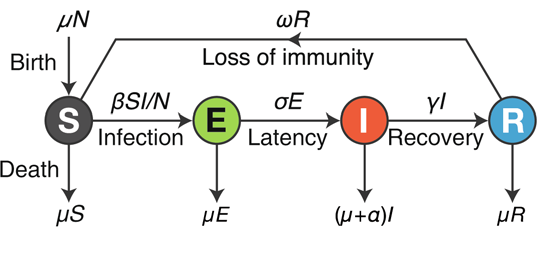
\includegraphics[width=\linewidth]{simpleSIRModel.png}
    \caption{Original Simple SIR Model (Benchmark) ~\cite{b19}}
    \label{fig:original_sir}
\end{figure}

\begin{figure}
    \centering
    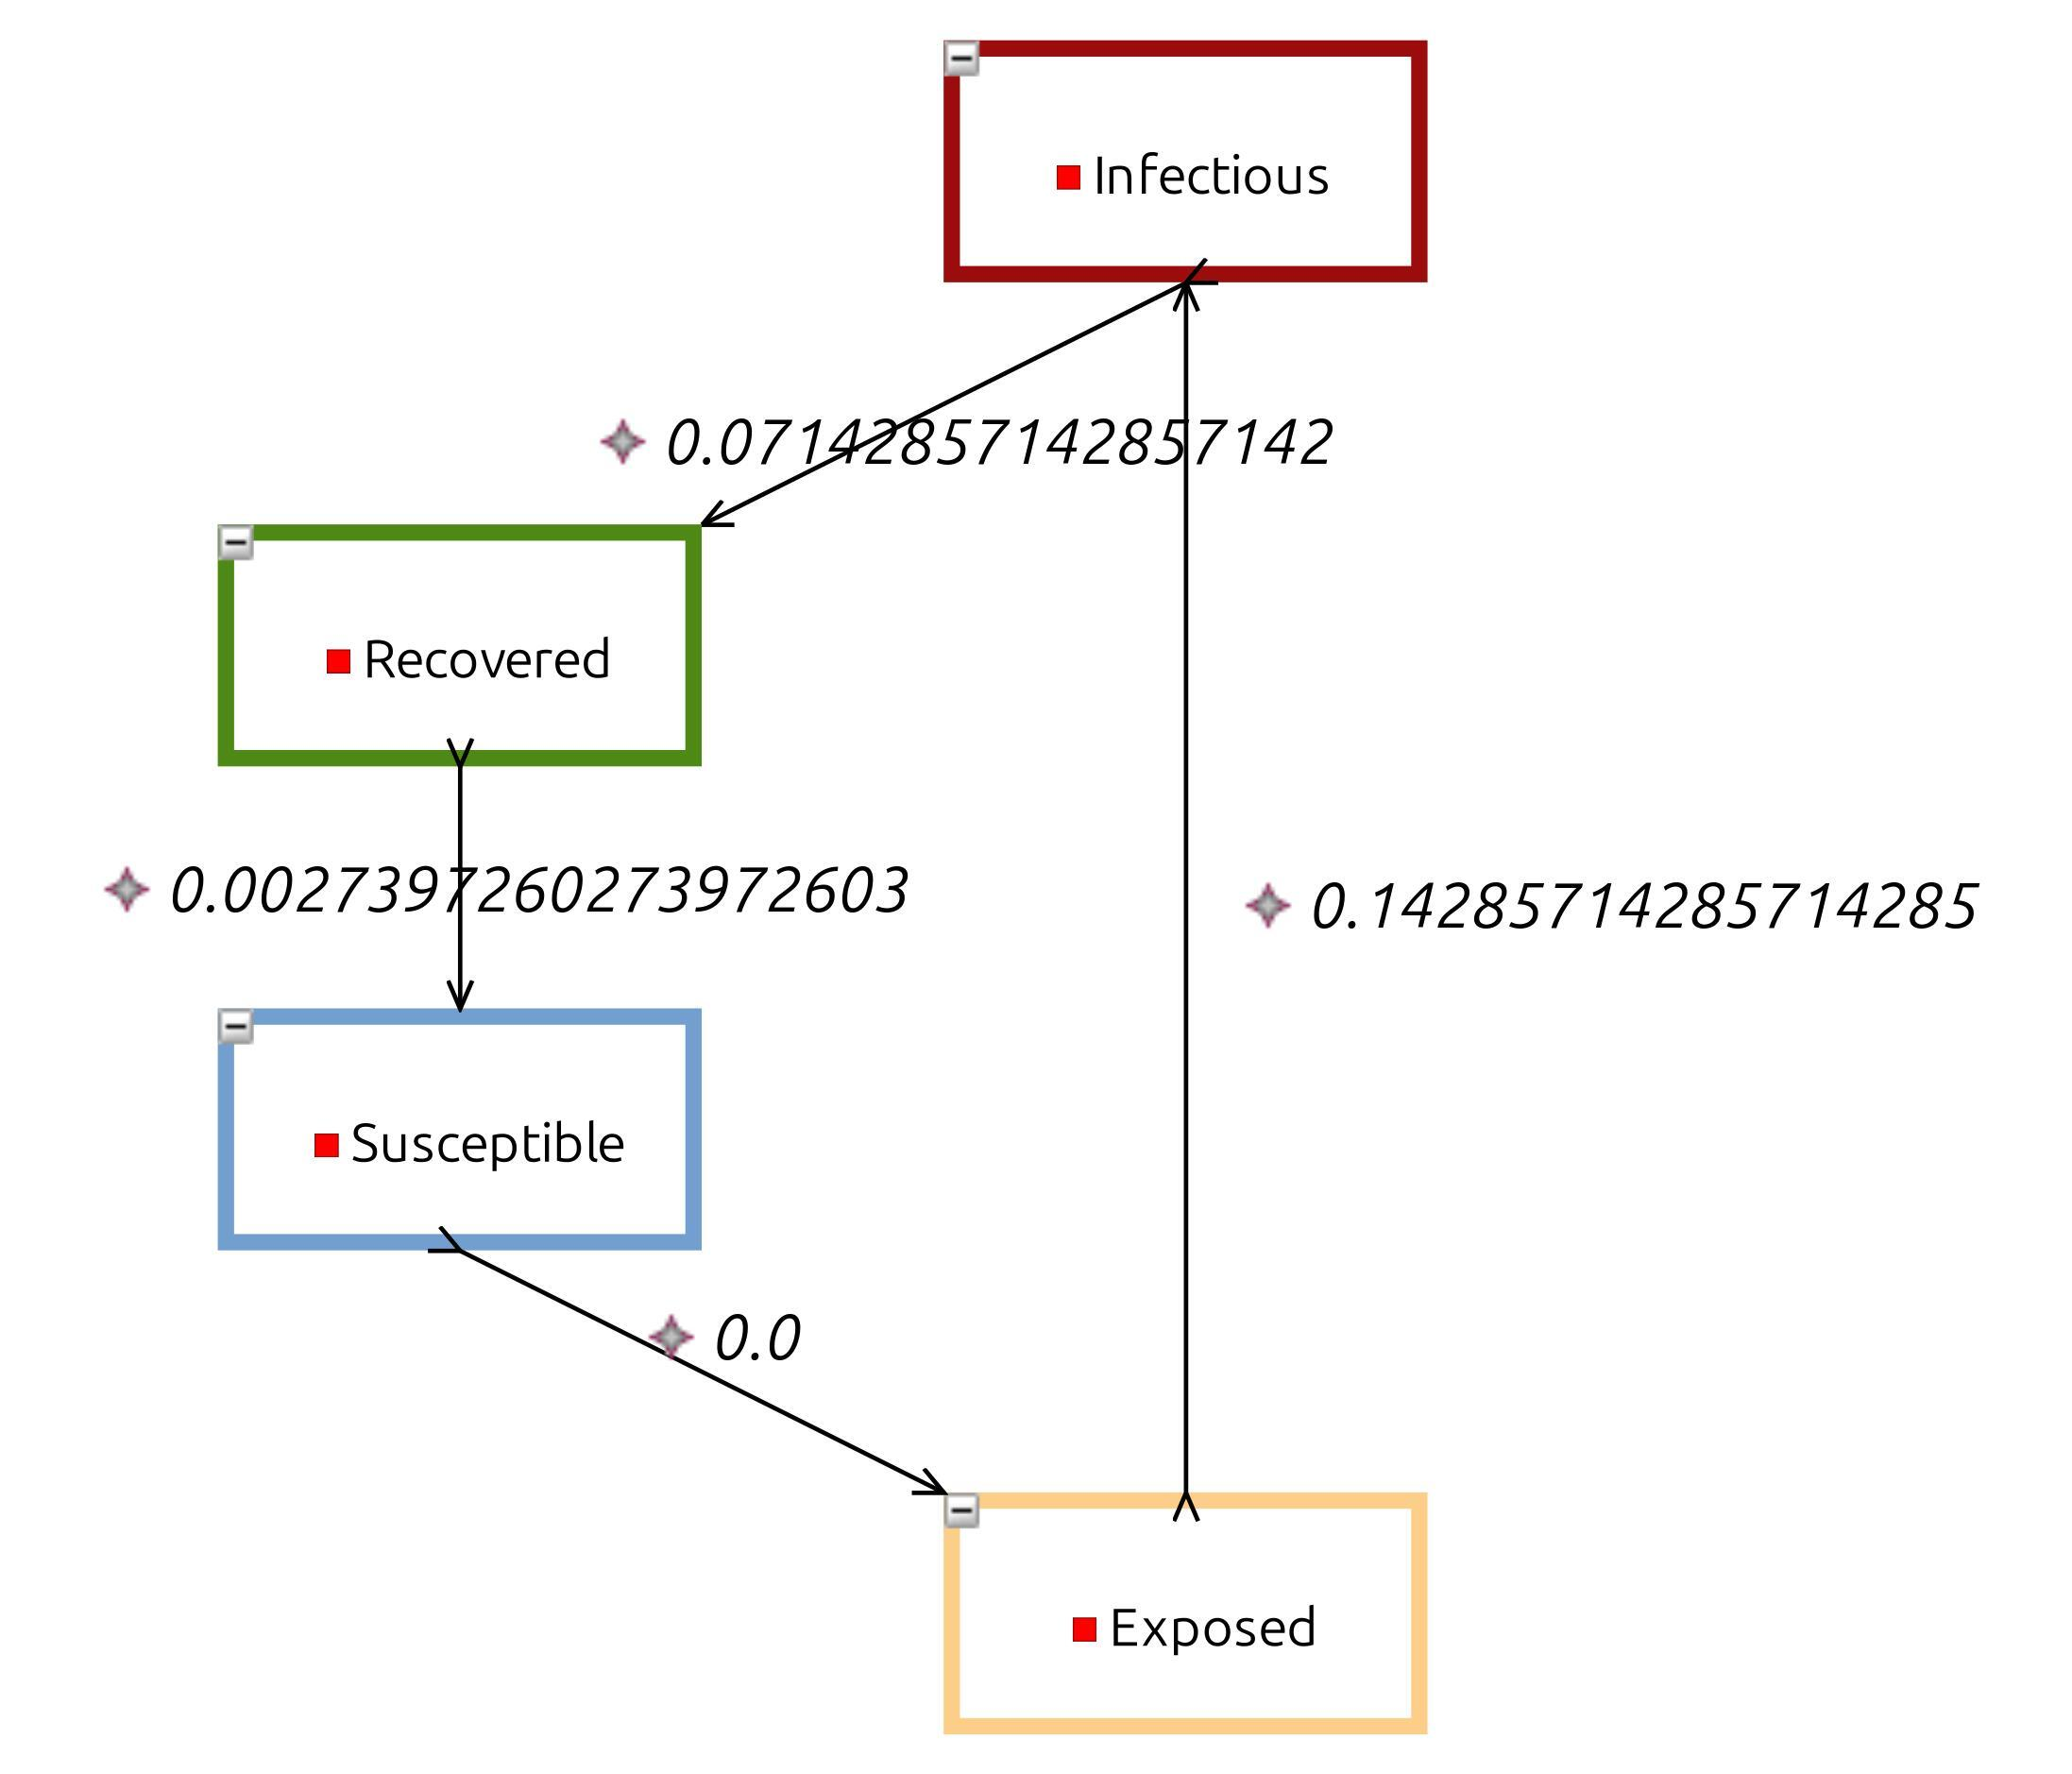
\includegraphics[width=\linewidth]{epimde-sir.jpg}
    \caption{Generated Simple SIR Model by the LLM in EpiMDE}
    \label{fig:generated_sir}
\end{figure}

Figures~\ref{fig:original_sir} and~\ref{fig:generated_sir} provide a visual comparison of the original Simple SIR model benchmark versus the LLM-generated version, which achieved a Precision of 1.000, Recall of 0.538, and F1-Score of 0.700. As observed, the generated model accurately captures the core SIR compartments and their primary transitions. However, it notably lacks the inflow and outflow elements present in the original, and the infection flow (originally contact-based) was implicitly handled as a skipped rate by the LLM (indicated by a 0 or placeholder in the XML, which is our model's way of flagging incomputable or unsupported calculations).

In conclusion, while the raw F1-Scores and Recall values might appear low, particularly when strict element-level counting is applied, it is crucial to recognize that a significant majority of the False Negatives represent the LLM's successful adherence to specified constraints and its intelligent flagging of features unsupported by the EpiMDE lite platform. This is a positive indicator of the pipeline's robustness in identifying and managing limitations. Nevertheless, the occasional mishaps, as observed in the COVID-19 model's False Positives, underscore the ongoing need for human oversight and potential areas for future refinement in complex model generation.

\section{Discussion}

Our experimental findings reveal both significant capabilities and important limitations of current LLM technology for automated epidemiological model generation. The successful generation of structurally correct \texttt{Seirmodel} XML files across varying complexity levels demonstrates the potential for LLMs to substantially reduce manual modeling effort while maintaining accuracy in domain-specific tasks.

\subsection{Key Findings and Implications}

Zero-shot metamodel prompting outperformed template-based approaches, demonstrating that formal constraint specification effectively guides LLM behavior in structured generation tasks. Multimodal input combining visual diagrams with tabular data proved essential, as images provide topological context while structured text supplies precise quantitative details. The ``reason-before-answer" strategy successfully addressed calculation limitations in multi-variable equations, indicating that explicit reasoning processes significantly improve LLM computational performance.

\subsection{Limitations and Challenges}

This study presents several important limitations that affect the generalizability and scope of our findings. First, the scale of our investigation is inherently limited, covering only three epidemiological scenarios (Simple SIR, COVID-19, and HIV transmission models) and utilizing a single LLM architecture (Gemini 2.5 Pro). While this focused approach allowed for deep investigation of prompt engineering techniques and detailed analysis of model generation quality, it restricts our ability to draw broad conclusions about LLM performance across the full spectrum of epidemiological modeling scenarios or different LLM architectures. The limited model diversity may not capture the full range of challenges present in epidemiological modeling, and single-LLM evaluation prevents assessment of approach generalizability across different language model capabilities and limitations.

Additional methodological limitations include mathematical reasoning constraints requiring explicit step-by-step guidance for complex calculations, high-quality input data requirements demanding domain expertise for proper model specification, and evaluation scope restricted to well-defined SEIR-type compartmental models. Our approach may not generalize to agent-based models, network-based epidemiological models, or other modeling paradigms outside the compartmental framework. Furthermore, the dependency on structured metamodel specifications and the EpiMDE platform's XML format constraints limit applicability to other epidemiological modeling frameworks and tools commonly used in the field.

\subsection{Future Directions}

Future work should explore automated validation integration for real-time feedback, specialized fine-tuned models for epidemiological domains, collaborative human-LLM workflows, and expansion to other scientific modeling domains to validate methodological generalizability.

\section{Conclusion}

This study presents the first comprehensive evaluation of LLMs for automated epidemiological model generation, demonstrating significant potential with important limitations. Our investigation reveals that LLMs can successfully translate natural language descriptions and visual diagrams into structured XML with high accuracy using appropriate prompt engineering.

Key contributions include: (1) comprehensive evaluation framework for domain-specific generation, (2) demonstration of zero-shot metamodel superiority over template-based approaches, (3) optimal multimodal input strategies, and (4) effective techniques for handling mathematical reasoning limitations. Findings indicate LLMs can significantly reduce manual modeling effort while maintaining accuracy, though mathematical reasoning limitations and structured input requirements highlight areas for continued development.

Our methodological frameworks provide foundational approaches for applying LLMs to specialized scientific domains with accuracy requirements. As LLM technology advances, automated model generation will become increasingly valuable for epidemiologists, potentially democratizing sophisticated modeling capabilities and accelerating emergency response times.

\section*{Acknowledgment}

This work was supported by the Wellcome Trust [226107/Z/22/Z]. The authors would like to thank the anonymous reviewers for their valuable feedback and suggestions that improved the quality of this paper.


\bibliographystyle{IEEEtran}
\bibliography{references}


\end{document}